\documentclass[10pt,nocopyrightspace]{sigplanconf}

% TODO: preprint      Remove this option only once the paper is in final form.
% TODO: 10pt, 11pt or nothing (default: 9pt)

\usepackage{amsmath}
\usepackage[T1]{fontenc}
\usepackage{hyperref}
\usepackage{graphicx}

% For draft paper only (TODO: remove)
\usepackage{blindtext}

\begin{document}

\special{papersize=8.5in,11in}
\setlength{\pdfpageheight}{\paperheight}
\setlength{\pdfpagewidth}{\paperwidth}

\titlebanner{banner above paper title}        % These are ignored unless
\preprintfooter{short description of paper}   % 'preprint' option specified.

\title{Hailstorm: Distributed stream processing with exactly once semantics}
\subtitle{CS240h Final Project, Spring 2014}

\authorinfo{Thomas Dimson \and Milind Ganjoo}
           {Stanford University}
           {tdimson@cs.stanford.edu \and mganjoo@cs.stanford.edu}

\maketitle

\begin{abstract}
In recent years, \textit{stream processing} has emerged as data analysis technique
to handle real-time applications where the latency of Hadoop is inappropriate. Many popular
systems, such as Twitter's Storm, provide a rigid platform for performing distributed
computations over the network. Storm-like systems typically provide at-least-once processing 
with state management left to the implementor. We present a novel distributed
stream processing framework, \textit{Hailstorm}\footnote{\url{https://github.com/hailstorm-hs/hailstorm}}, which provides a platform to perform distributed
commuative monoidic operations on a stream of data in Haskell. By restricting the 
class of computation, our system is provides exactly-once semantics 
with little performance loss or added complexity. 

\end{abstract}

% \keywords
% keyword1, keyword2

\section{Introduction}


\section{Related Work}
In Exactly Once Semantics~\cite{jackson2014}, Jackson describes some stuff.

We base our system on the design of Storm~\cite{storm}

Also, let's talk about Google's MillWheel system~\cite{millwheel}

\section{Foundational Systems}
\subsection{Apache Kafka}
Kafka~\cite{kafka} is fantastic.

Haskakafka \footnote{\url{http://hackage.haskell.org/package/haskakafka}}

\subsection{Apache Zookeeper}
Zookeeper~\cite{zookeeper} is the best.


\section{Hailstorm Overview}
Let's talk about how the components fit together 
(spouts, bolts, etc.)

\begin{figure}
\centering
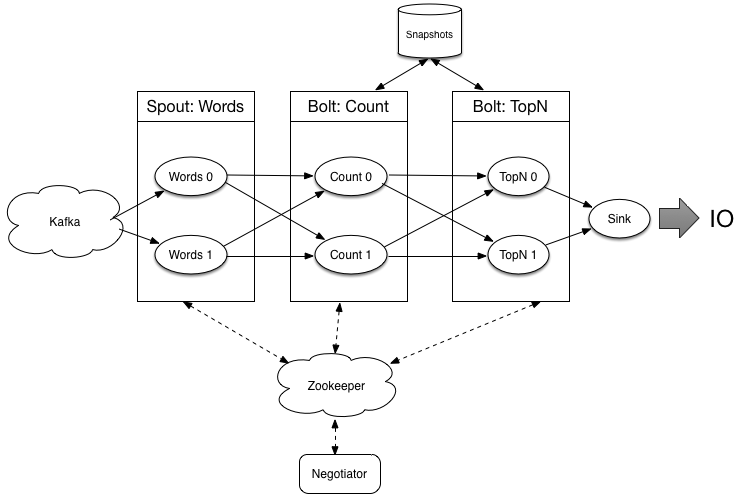
\includegraphics[width=0.5\textwidth]{images/architecture.png}
\caption{An example Hailstorm topology for word counts}
\end{figure}

\section{Next Steps}

\section{Conclusion}

\bibliography{hailstorm}{}
\bibliographystyle{abbrvnat}

\end{document}
